\documentclass[a4 paper, 12pt]{article}
\usepackage[brazilian]{babel}
\usepackage[utf8]{inputenc}
\usepackage[T1]{fontenc}
\usepackage{minted}
\usepackage{anysize}
\usepackage{graphicx}
\marginsize{3cm}{3cm}{2cm}{2cm}
\usemintedstyle{tango}
\newminted{cpp}{linenos, mathescape, frame=topline, numberblanklines=false}
\newmint{cpp}{frame=single}
\usepackage{amsfonts}
\usepackage{amssymb}
\usepackage{algorithmic}
\usepackage[brazilian]{algorithm}
\renewcommand{\algorithmicrequire}{\textbf{Entrada:}}
\renewcommand{\algorithmicensure}{\textbf{Saída:}}
\renewcommand{\algorithmicend}{\textbf{fim}}
\renewcommand{\algorithmicif}{\textbf{se}}
\renewcommand{\algorithmicthen}{\textbf{então}}
\renewcommand{\algorithmicelse}{\textbf{else}}
\renewcommand{\algorithmicelsif}{\algorithmicelse\ \algorithmicif}
\renewcommand{\algorithmicendif}{\algorithmicend\ \algorithmicif}
\renewcommand{\algorithmicfor}{\textbf{para}}
\renewcommand{\algorithmicforall}{\textbf{para todos}}
\renewcommand{\algorithmicdo}{\textbf{faça}}
\renewcommand{\algorithmicendfor}{\algorithmicend}
\renewcommand{\algorithmicwhile}{\textbf{enquanto}}
\renewcommand{\algorithmicendwhile}{\algorithmicend}
\renewcommand{\algorithmicloop}{\textbf{loop}}
\renewcommand{\algorithmicendloop}{\algorithmicend\ \algorithmicloop}
\renewcommand{\algorithmicrepeat}{\textbf{repita}}
\renewcommand{\algorithmicuntil}{\textbf{enquanto}}
\renewcommand{\algorithmicprint}{\textbf{imprima}}
\renewcommand{\algorithmicreturn}{\textbf{retorne}}
\renewcommand{\algorithmictrue}{\textbf{verdadeiro}}
\renewcommand{\algorithmicfalse}{\textbf{falso}}


\renewcommand{\theFancyVerbLine}{
  \sffamily\textcolor[rgb]{0.5,0.5,0.5}{\scriptsize\arabic{FancyVerbLine}}}

\def\linha#1{
  \hbox to \hsize{
      \vbox{\centering #1}}
      \vspace{4mm}}

\begin{document}
\begin{titlepage}
\thispagestyle{empty}
\linha{\Huge \textbf {Universidade de São Paulo}}
\vspace{40mm}

%TÌtulo
\linha{\large PCS5730: Projeto e Técnicas de Construção de
  Compiladores\\}
\vspace{10mm}
\linha{\LARGE \textbf{\emph{There and back again}:\\Convertendo
    aut\^omatos para gram\'aticas}}
\vspace{50mm}
\linha{\large \textbf{Lucas Virgili}}

\vspace{50mm}
\linha{\large 1º Semestre de 2014}


\end{titlepage}
\tableofcontents
\newpage

\section{Resumo}
Neste trabalho, propomos o desenvolvimento de um conjunto de
ferramentas que ser\'a usado para obter uma gram\'atica equivalente a
um aut\^omato, representado em forma de matriz.

\section{Introdu\c c\~ao}

\section{Gram\'aticas e aut\^omatos}

\section{Ferramenta para obter a gram\'atica a partir de um
  aut\^omato}
Neste trabalho, desenvolveremos duas ferramentas: a primeira, dada uma
matriz representando um aut\^omato, computa a representa\c c\~ao do
aut\^omato em express\~ao regular; a segunda converte uma express\~ao
regular em uma gram\'atica na nota\c c\~ao escolhida pelo
usu\'ario. Logo, utilizando as duas ferramentas em um
\emph{pipeline}, obtemos uma gram\'atica equivalente ao aut\^omato. A
figura \ref{fig:1} representa o processo.

\begin{figure}[H]
  \centering
  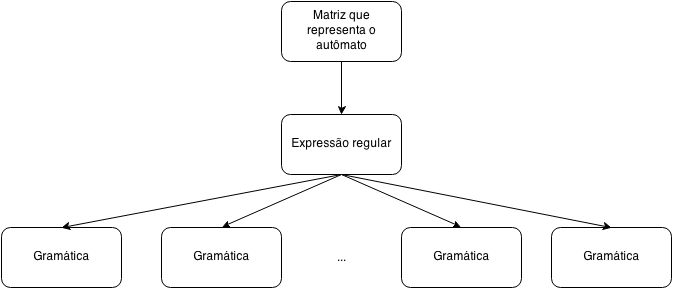
\includegraphics[width=0.8\textwidth]{estruturabranco.png}
  \caption{Oten\c c\~ao de gram\'aticas a partir do aut\^omato}
  \label{fig:1}
\end{figure}

\subsection{Obtendo a express\~ao regular}
Sejam $\{q_1, q_2, \ldots, q_k\}$ os estados do aut\^omato.

A ideia \'e usar um tipo de ``indu\c c\~ao'': seja $R_{i,j}^k$
a express\~ao regular para as entradas indo do estado $i$ ao estado
$j$, usando somente os $k$ primeiros estados do aut\^omato.

Para cada par $i, j$, suponha que $R_{i,j}$ represente a express\~ao
de $q_i$ at\'e $q_j$, mas sem usar o estado $q_k$. Agora, se pudermos
usar o estado $q_k$, podemos montar o novo $R$:
\begin{equation}
  \label{eq:1}
  R_{i,j}^{k} = R_{i,j}^{k-1} + R_{i,k}^{k-1} . R_{k,k}^{k-1*}. R_{k,j}^{k-1}
\end{equation}

Isso quer dizer que, para irmos de $i$ a $j$, podemos usar o que j\'a
sab\'iamos ou ir de $i$ at\'e o estado $k$, ficar em \emph{loop} em
$k$ e depois irmos de $k$ at\'e o estado $j$.

O algoritmo, em ``pseudo python'':
\begin{minted}[mathescape, linenos=true, frame=lines]{python}
# Automato Sigma:
# n estados
# R matriz

# Inicializacao:
for i in range(1, n):
    for j in range(1, n):
        if i == j:
            R[i][j][0] = epsilon
        else:
            R[i][j][0] = nada
        for terminal in Sigma:
            if transicao(i, terminal, j):
                R[i][j][0] = R[i][j][0] + terminal

# Inducao
for k in range(1, n):
    for i in range(1, n):
        for j in range(1, n):
            R[i][j][k] = R[i][j][k-1] + R[i][k][k-1]
            . estrela_kleene(R[k][k][k-1]) . R[k][j][k-1]

# Regex
inicio = find_inicio(Sigma)
for i in range(1, n):
    if is_final(i):
        regex = regex + R[inicio][i][n]
\end{minted}

Note que o algoritmo n\~ao gera a express\~ao regular mais bonita.

\section{Conclus\~ao}

\newpage
\section{Bibliografia}
http://cs.stackexchange.com/questions/2016/how-to-convert-finite-automata-to-regular-expressions
\end{document}